% ─────────────────────────────────────────────────────────────────────────────
% chapters/ch3_implementation.tex — Chapter 3: System Implementation
% ─────────────────────────────────────────────────────────────────────────────

\chapter{System Implementation}

This chapter presents the concrete realisation of \textit{Mobile Match Algeria}. Each major subsystem is described in turn: the development environment, the data aggregation module, the REST API, the recommendation engine, the key user interface screens, the security mechanisms, and the deployment configuration.

\section{Development Environment}

Table~\ref{tab:dev-env} describes the hardware and software environment used throughout the development of this project.

\begin{table}[H]
  \caption{Development environment}
  \label{tab:dev-env}
  \centering\small
  \begin{tabular}{|p{4cm}|p{11cm}|}
    \hline
    \textbf{Component}  & \textbf{Details} \\
    \hline
    Operating system    & Windows 11 Pro (Build 22631) \\
    \hline
    Runtime             & Node.js 20.11.0 LTS \\
    \hline
    Package manager     & npm 10.2.4 \\
    \hline
    Framework           & Next.js 16.2.3 \\
    \hline
    Language            & TypeScript 5.x (strict mode) \\
    \hline
    ORM                 & Prisma 7.x \\
    \hline
    Database            & SQLite (via Prisma driver adapter) \\
    \hline
    IDE                 & Visual Studio Code 1.89 \\
    \hline
    Version control     & Git 2.44, repository hosted on GitHub \\
    \hline
    Browser testing     & Google Chrome 124, Mozilla Firefox 125 \\
    \hline
  \end{tabular}
\end{table}

The project was initialised with \texttt{create-next-app} and immediately configured with strict TypeScript, ESLint, and Prisma. All sensitive configuration (database path, session secret, base URL) is stored in a \texttt{.env} file excluded from version control.

\section{Data Aggregation Module}

\subsection{Scraper Architecture}

The data aggregation module resides in \texttt{src/lib/scraper/} and follows a strict separation of concerns. Three per-operator scrapers (\texttt{djezzy.ts}, \texttt{ooredoo.ts}, \texttt{mobilis.ts}) are each responsible only for fetching and parsing their respective operator's plan page and returning a normalised array of raw offer objects. A central orchestrator (\texttt{index.ts}) coordinates all three scrapers and handles every database operation, deactivation decision, and notification dispatch.

\subsection{Scraping Algorithm}

Figure~\ref{fig:scraper-algo} presents the algorithm executed by the orchestrator for a single operator.

\begin{figure}[H]
\centering
\begin{tikzpicture}[
  box/.style={rectangle, draw=black!70, fill=gray!6, rounded corners=3pt,
              minimum width=13cm, minimum height=0.7cm, align=left,
              font=\small, inner sep=5pt},
  head/.style={rectangle, draw=black, fill=black!85, rounded corners=3pt,
               minimum width=13cm, minimum height=0.7cm, align=left,
               font=\small\bfseries\color{white}, inner sep=5pt},
  arrow/.style={-{Stealth[length=4pt]}, thick, gray!70},
  node distance=0.18cm
]
  \node[head]  (h)  {Algorithm: Automated Scraping Pipeline \hfill \textit{Input: operator, scraper\_fn \quad Output: ScrapeResult}};
  \node[box, below=of h]  (s1)  {\textbf{1.} Record \textit{startedAt}; create ScrapeLog with status = RUNNING};
  \node[box, below=of s1] (s2)  {\textbf{2.} Invoke \textit{scraper\_fn}: fetch operator page (HTTP GET), parse HTML, normalise attributes};
  \node[box, below=of s2] (s3)  {\textbf{3.} Filter out offers missing all data, voice, and SMS values};
  \node[box, below=of s3] (s4)  {\textbf{4.} For each valid offer:};
  \node[box, below=of s4] (s4a) {\quad\quad \textbf{a.} Compute slug = slugify(offer.name)};
  \node[box, below=of s4a](s4b) {\quad\quad \textbf{b.} If slug exists in DB $\Rightarrow$ UPDATE record; else $\Rightarrow$ INSERT \& notify users};
  \node[box, below=of s4b](s5)  {\textbf{5.} Per-family deactivation: group scraped offers by source URL (one URL = one plan family)};
  \node[box, below=of s5] (s5a) {\quad\quad For each non-empty family: set isActive = false for DB offers of that URL absent from scrape};
  \node[box, below=of s5a](s6)  {\textbf{6.} Update ScrapeLog: status = SUCCESS, duration, offersAdded, offersUpdated};
  \node[box, below=of s6] (s7)  {\textbf{7.} Return ScrapeResult \quad\quad \textit{On error: status = FAILED, log errorMessage}};

  \foreach \a/\b in {h/s1, s1/s2, s2/s3, s3/s4, s4/s4a, s4a/s4b, s4b/s5, s5/s5a, s5a/s6, s6/s7}
    \draw[arrow] (\a.south) -- (\b.north);
\end{tikzpicture}
\caption{Algorithm of the automated scraping pipeline}
\label{fig:scraper-algo}
\end{figure}

A key precision mechanism is the \textbf{per-family deactivation} at step~5. Rather than comparing global offer counts — which would incorrectly block cleanup when the total scrape count differs from the database total due to unrelated family changes — the orchestrator groups the scraped offers by their source URL. Each URL corresponds to exactly one plan family (for example, one page for LEGEND, one for CAMPUCE, one for DjezzyNet). For each family that returned at least one offer in the current run, any database record sharing that source URL but absent from the current scrape is marked inactive. This detects removed plans precisely at the family level, independently of what other families returned in the same run.

\subsection{Data Normalisation Pipeline}

Each operator presents plan data in a different format. The normalisation pipeline applies the following transformations before storing any record: data volumes expressed in megabytes are converted to gigabytes; plan names are trimmed and stripped of promotional suffixes; missing voice or SMS values are defaulted to zero; the plan type (prepaid, postpaid, data-only) is inferred from page context when not explicitly stated; and a unique slug is generated from the normalised name. The pipeline outputs objects that conform to the \texttt{Offer} schema defined in Prisma.

\subsection{Cron Automation}

The scraper is triggered automatically every day at 03:00~AM Algeria time (UTC+1) using the \texttt{node-cron} library, registered at server startup via the Next.js instrumentation hook. Administrators may also initiate a manual run from the admin dashboard at any time. After each successful scrape cycle, the orchestrator runs the recommendation engine against all active user profiles and dispatches personalised notifications to users whose top-matched plan has a score of 75 or above.

\section{Backend --- REST API}

\subsection{API Route Structure}

All API routes are implemented as Next.js App Router route handlers under \texttt{src/app/api/}. Each file exports named async functions corresponding to HTTP methods (\texttt{GET}, \texttt{POST}, \texttt{PATCH}, \texttt{DELETE}). Route-level middleware checks for a valid session before executing any protected operation. Table~\ref{tab:api-routes} summarises all available routes.

\begin{table}[H]
  \caption{API route map}
  \label{tab:api-routes}
  \centering\small
  \begin{tabular}{|p{4.2cm}|p{2.6cm}|p{7.0cm}|}
    \hline
    \textbf{Route} & \textbf{Methods} & \textbf{Function} \\
    \hline
    \texttt{/api/offers}          & GET                & List and filter active offers; fetch specific offers by ID list for comparison (bypasses isActive filter) \\
    \hline
    \texttt{/api/offers/[id]}     & GET, PATCH, DELETE & Retrieve, update, or delete a single offer (admin only) \\
    \hline
    \texttt{/api/saved-offers}    & GET, POST          & List saved offer IDs; toggle save/unsave \\
    \hline
    \texttt{/api/recommendations} & POST               & Run scoring engine; return top-3 matched plans \\
    \hline
    \texttt{/api/notifications}   & GET, PATCH, DELETE & List, mark-all-read, or delete a notification \\
    \hline
    \texttt{/api/profile}         & GET, PUT           & Retrieve or update the user's usage profile \\
    \hline
    \texttt{/api/admin/stats}      & GET                & Platform statistics (users, active offers, scrape sessions, operator health) \\
    \hline
    \texttt{/api/admin/scrape}     & POST               & Trigger a full scrape run across all three operators \\
    \hline
    \texttt{/api/stats}           & GET                & Public statistics (offer count, operators) \\
    \hline
  \end{tabular}
\end{table}

\subsection{Cross-Operator Comparison Routing}

One non-trivial design decision in the offers route concerns the comparison feature. When a user selects plans from different operators and navigates to the comparison page, the IDs are passed as a query parameter (\texttt{?ids=a,b,c}). The \texttt{/api/offers} handler detects this parameter and executes a direct lookup by ID list, deliberately bypassing the \texttt{isActive} filter that applies to the normal listing path. This ensures that saved plans remain comparable even if a subsequent scrape run has marked them inactive.

\subsection{Authentication}

User authentication is implemented with \textit{NextAuth.js} using the Credentials provider. Passwords are hashed with bcrypt at registration and verified at sign-in. Sessions are JWT-based with a 30-day expiry. The \texttt{role} field (\texttt{USER} or \texttt{ADMIN}) is embedded in the session token and verified at the start of every admin-gated route handler.

\section{Recommendation Engine}

\subsection{Scoring Model}

The recommendation engine is implemented in \texttt{src/lib/recommendation.ts}. It applies a 100-point composite score to each active offer using eight weighted dimensions, as listed in Table~\ref{tab:scoring}.

\begin{table}[H]
  \caption{Scoring dimensions of the recommendation engine}
  \label{tab:scoring}
  \centering\small
  \begin{tabular}{|p{3.5cm}|p{9.5cm}|>{\centering\arraybackslash}p{1.5cm}|}
    \hline
    \textbf{Dimension} & \textbf{Scoring logic} & \textbf{Max pts} \\
    \hline
    Budget fit           & Ratio of offer price to declared budget; full score if well within budget, zero if more than 15\,\% over & 25 \\
    \hline
    Data fit             & Ratio of included data to declared need; full score for unlimited data & 25 \\
    \hline
    Voice fit            & Ratio of included minutes to declared need; full score for unlimited calls & 15 \\
    \hline
    SMS fit              & Ratio of included SMS to declared need; weighted low because OTT messaging apps have largely replaced SMS in Algeria & 5 \\
    \hline
    Value bonus          & Data-per-Dinar ratio (MB per DA): rewards cost-effectiveness; highest-weighted bonus dimension & 15 \\
    \hline
    Feature bonus        & Presence of streaming, social media, night bonus, or roaming in plan description & 5 \\
    \hline
    Validity fit         & Monthly plans ($\geq$30 days) score highest; weekly plans partial; daily minimal & 5 \\
    \hline
    Type / network match & Direct match to declared preferred type adds points; mismatch subtracts 5 pts & 5 \\
    \hline
    \textbf{Total}       & & \textbf{100} \\
    \hline
  \end{tabular}
\end{table}

\noindent\textbf{Dimension weight rationale.} Budget and data each receive the maximum 25~points because they represent the two constraints that Algerian mobile users consistently cite as primary when selecting a plan: affordability and data volume \parencite{GSMA2024, ARPCE2024}. Voice minutes receive 15~points, reflecting their continued relevance for calls within Algeria despite declining usage trends. The value bonus (15~points) is the highest-weighted secondary dimension, rewarding cost-efficiency — a critical differentiator in a price-sensitive prepaid market. SMS is weighted at only 5~points because over-the-top messaging applications have largely supplanted SMS in Algerian consumer behaviour \parencite{GSMA2024}. The remaining three dimensions (feature set, validity, type/network) each receive 5~points as contextual tiebreakers.

\subsection{Recommendation Algorithm}

Figure~\ref{fig:rec-algo} presents the complete recommendation algorithm.

\begin{figure}[H]
\centering
\begin{tikzpicture}[
  box/.style={rectangle, draw=black!70, fill=gray!6, rounded corners=3pt,
              minimum width=13cm, minimum height=0.7cm, align=left,
              font=\small, inner sep=5pt},
  head/.style={rectangle, draw=black, fill=black!85, rounded corners=3pt,
               minimum width=13cm, minimum height=0.7cm, align=left,
               text width=12.2cm,
               font=\small\bfseries\color{white}, inner sep=5pt},
  arrow/.style={-{Stealth[length=4pt]}, thick, gray!70},
  node distance=0.18cm
]
  \node[head]  (h)  {Algorithm: Multi-Criteria Plan Recommendation \\ \normalfont\textit{\scriptsize Input: offers[ ], profile \quad Output: Recommendation[ ]}};
  \node[box, below=of h]  (s1) {\textbf{1.} Pre-filter: discard offers where price $>$ budget $\times$ 1.15};
  \node[box, below=of s1] (s2) {\textbf{2.} For each remaining offer, compute score (clamped to [0, 100]):};
  \node[box, below=of s2] (s2a){\quad\quad \textbf{a.} Budget fit (25 pts): inversely proportional to price / budget ratio};
  \node[box, below=of s2a](s2b){\quad\quad \textbf{b.} Data fit (25 pts): proportional to dataGB / profile.dataGB};
  \node[box, below=of s2b](s2c){\quad\quad \textbf{c.} Voice fit (15 pts): proportional to voiceMinutes / profile.voiceMinutes};
  \node[box, below=of s2c](s2d){\quad\quad \textbf{d.} SMS fit (5 pts): proportional to smsCount / profile.smsCount (low weight: OTT apps dominate)};
  \node[box, below=of s2d](s2e){\quad\quad \textbf{e.} Value bonus (15 pts): data-per-Dinar ratio (MB per DA)};
  \node[box, below=of s2e](s2f){\quad\quad \textbf{f.} Feature bonus (5 pts): streaming, social, night, roaming keywords};
  \node[box, below=of s2f](s2g){\quad\quad \textbf{g.} Validity fit (5 pts): $\geq$30 days = 5 pts; $\geq$7 days = 3 pts; else 1 pt};
  \node[box, below=of s2g](s2h){\quad\quad \textbf{h.} Type / network match (5 pts): mismatch subtracts 5 pts};
  \node[box, below=of s2h](s3) {\textbf{3.} Sort scored offers descending by score};
  \node[box, below=of s3] (s4) {\textbf{4.} Operator diversity check: if top-3 are all from same operator $\Rightarrow$};
  \node[box, below=of s4] (s4a){\quad\quad swap \#3 with best different-operator offer within 15\,\% of \#3 score};
  \node[box, below=of s4a](s5) {\textbf{5.} Return top-N results with matchReasons[ ] and mismatches[ ]};

  \foreach \a/\b in {h/s1, s1/s2, s2/s2a, s2a/s2b, s2b/s2c, s2c/s2d, s2d/s2e, s2e/s2f, s2f/s2g, s2g/s2h, s2h/s3, s3/s4, s4/s4a, s4a/s5}
    \draw[arrow] (\a.south) -- (\b.north);
\end{tikzpicture}
\caption{Multi-criteria recommendation algorithm}
\label{fig:rec-algo}
\end{figure}

The diversity check at step~4 prevents the engine from returning three plans from the same operator when the user's profile happens to strongly match that operator's catalogue. This ensures that recommendations offer a meaningful choice across operators.

\subsection{Triggering Recommendations}

The engine is called from two distinct contexts. The first is the \texttt{/api/recommendations} route handler, which executes the algorithm synchronously in response to an explicit user request from the recommendations page. The second is the scraper orchestrator, which runs the engine in batch after each successful scrape cycle to generate proactive notification recommendations for all registered users who have a saved profile.

\subsection{Operator Affinity Personalisation}

In addition to the content-based scoring described above, the engine incorporates a lightweight behavioural signal derived from each user's saved offers. When the \texttt{/api/recommendations} route is called for an authenticated user, the server retrieves the user's complete saved-offer list and counts how many saved offers belong to each operator. This produces an \textit{operator affinity map} — a dictionary keyed by operator identifier with the count of saved offers as the value.

After the initial content-based scoring and sorting, each offer receives an affinity boost equal to $\min(5,\; \text{count} \times 2)$~points, where \textit{count} is the number of the user's saved offers from that operator. The boost is capped at 5~points out of 100 to ensure that content-based fit always dominates: no offer can move from a poor match to a good match on affinity alone. The results are re-sorted after the boost is applied. If an offer receives any affinity boost, its match-reason panel displays the indicator \guillemotleft{}Matches your preferred operator\guillemotright{} so the personalisation is visible and not hidden from the user.

This approach follows the implicit-feedback paradigm in recommender systems research, where user actions such as saves, clicks, or purchase history serve as proxies for preference in the absence of explicit ratings \parencite{hu2008collaborative}. The limitation of this signal — that saving an offer does not unambiguously indicate operator loyalty — is explicitly acknowledged in Chapter~4.

\section{Frontend --- Key Interfaces}

The application comprises six primary screens covering the full user journey from discovery to account management. This section describes each interface and illustrates its appearance in the running application.

\subsection{Home Page and Offer Browsing}

The home page (Figure~\ref{fig:ss-home}) serves as the entry point for unauthenticated users. It presents a language selector (English, French, or Arabic), four feature highlight tiles (Compare Plans, Personalised Recommendations, Save Favourites, Live Data), and the three operator logos. Selecting a language stores the preference and redirects immediately to the offers catalogue. Authenticated users bypass this screen entirely and are redirected directly to the offers page.

\begin{figure}[H]
  \centering
  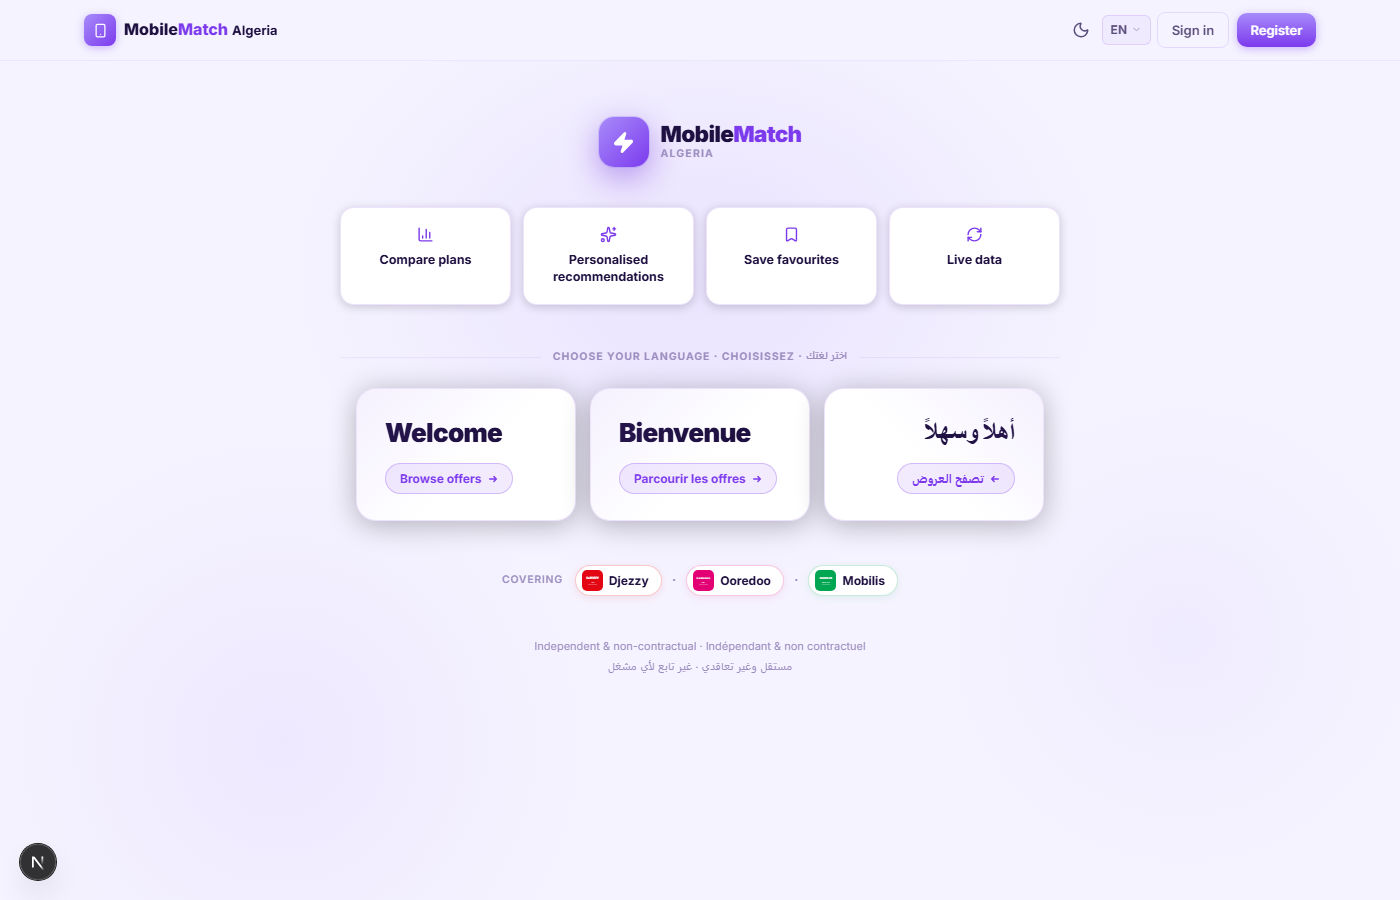
\includegraphics[width=0.95\textwidth]{images/screenshot_home}
  \caption{Home page of Mobile Match Algeria}
  \label{fig:ss-home}
\end{figure}

\subsection{Offers Page}

The offers page (Figure~\ref{fig:ss-offers}) is the application's main discovery surface. It renders a grid of offer cards using the shared \texttt{OfferCard} component, with staggered entrance animations. Operator filter tabs are rendered at the top of the page, and a collapsible advanced filter panel provides range sliders for maximum price and minimum data together with network generation toggles. When a user selects plans for comparison, a fixed-bottom sticky bar appears (Figure~\ref{fig:compare-bar}) displaying the selection count and a navigation button.

\begin{figure}[H]
  \centering
  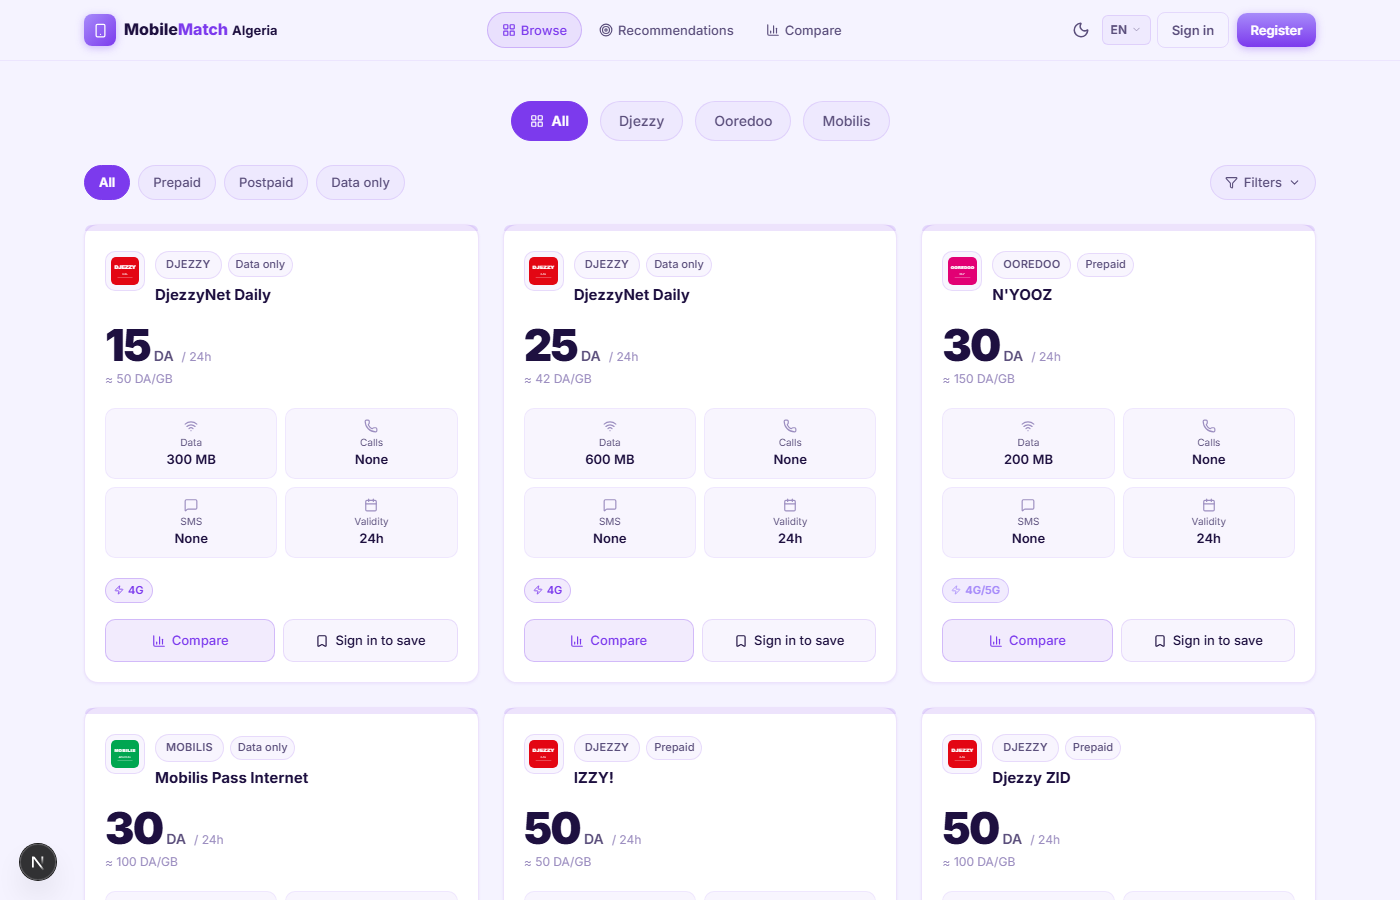
\includegraphics[width=0.95\textwidth]{images/screenshot_offers}
  \caption{Offers page showing plan catalogue with operator filter tabs}
  \label{fig:ss-offers}
\end{figure}

\begin{figure}[H]
  \centering
  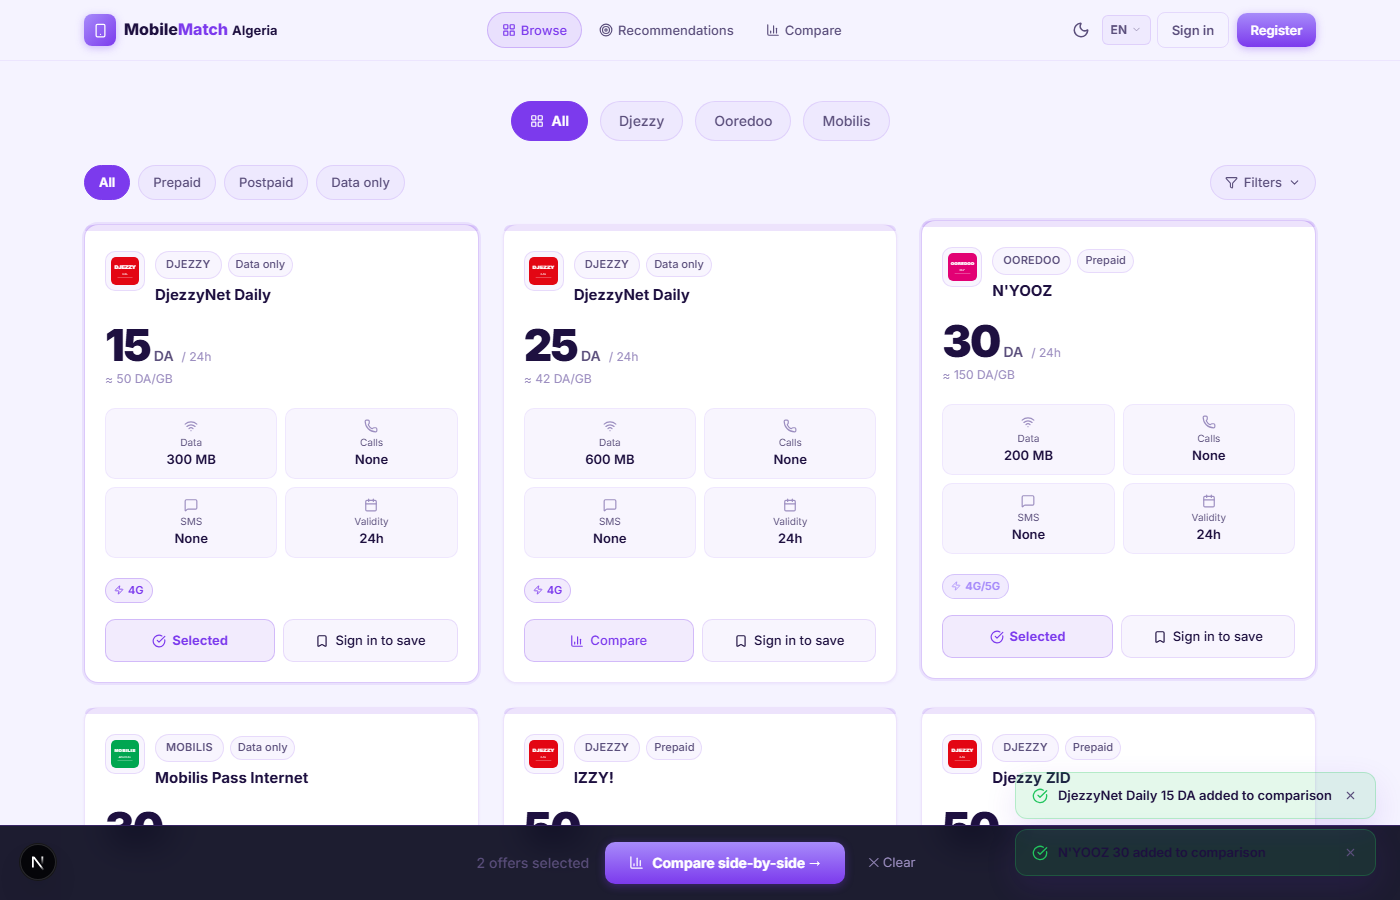
\includegraphics[width=0.95\textwidth]{images/compare_bar}
  \caption{Sticky comparison bar --- appears at the bottom when plans are selected}
  \label{fig:compare-bar}
\end{figure}

\subsection{Comparison Page}

The comparison page (Figure~\ref{fig:ss-compare}) reads the plan IDs from the URL query string and fetches the corresponding offers from the \texttt{/api/offers?ids=...} endpoint. It renders a structured side-by-side table where the best value for each row is highlighted in the accent colour, covering six attributes: type, price, data, voice, SMS, and validity.

\begin{figure}[H]
  \centering
  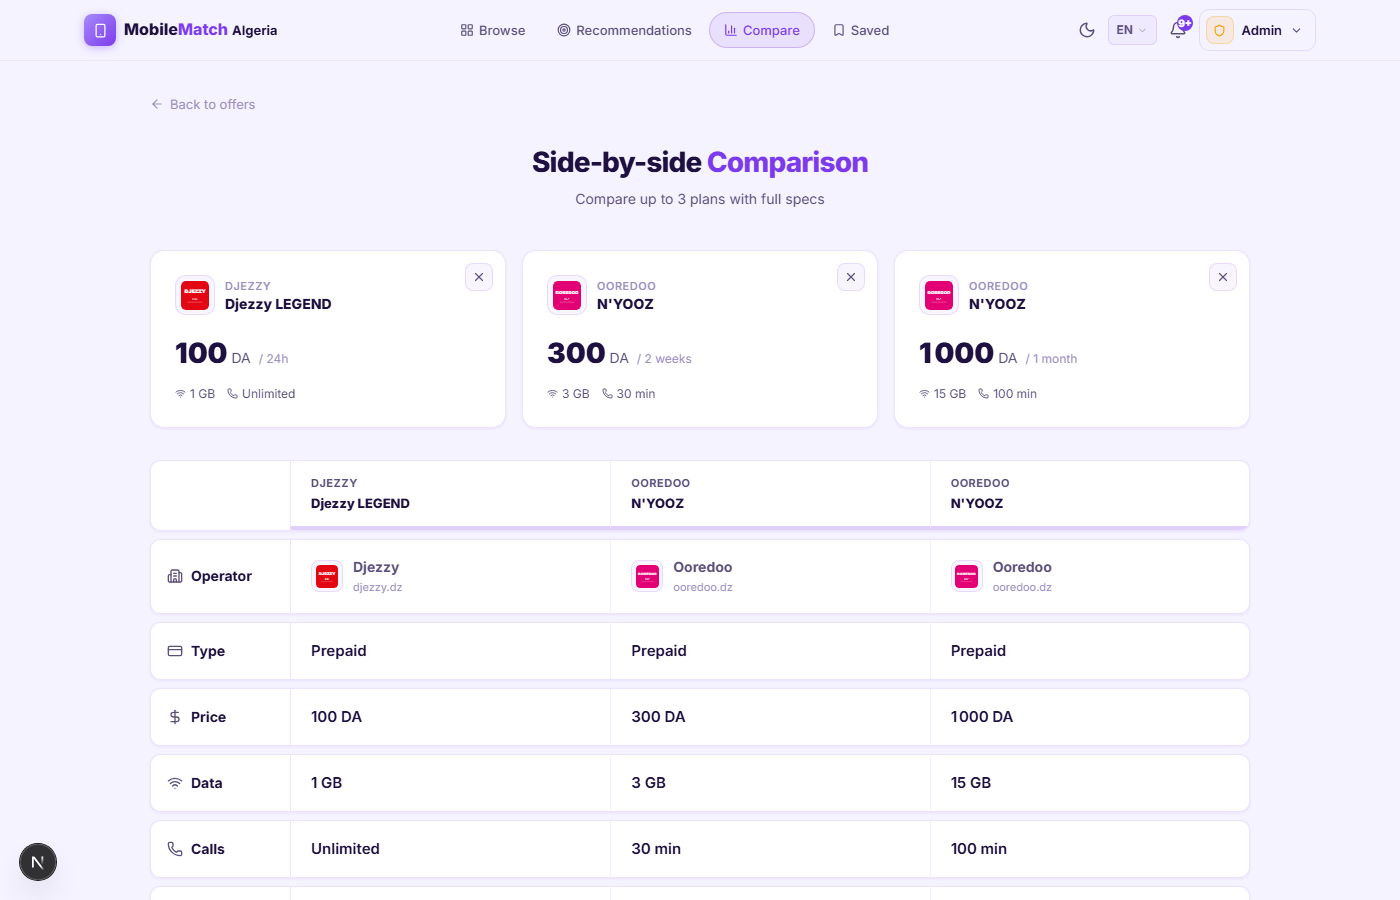
\includegraphics[width=0.95\textwidth]{images/screenshot_compare}
  \caption{Side-by-side comparison page with best-value row highlighting}
  \label{fig:ss-compare}
\end{figure}

\subsection{Recommendations Page}

The recommendations page (Figure~\ref{fig:ss-recommend}) presents a usage profile form with range sliders for budget, data, voice, and SMS, and toggle buttons for preferred plan type and network generation. On submission, the form sends a POST request to \texttt{/api/recommendations} and renders the top three scored plans with their composite scores and the specific match reasons.

\begin{figure}[H]
  \centering
  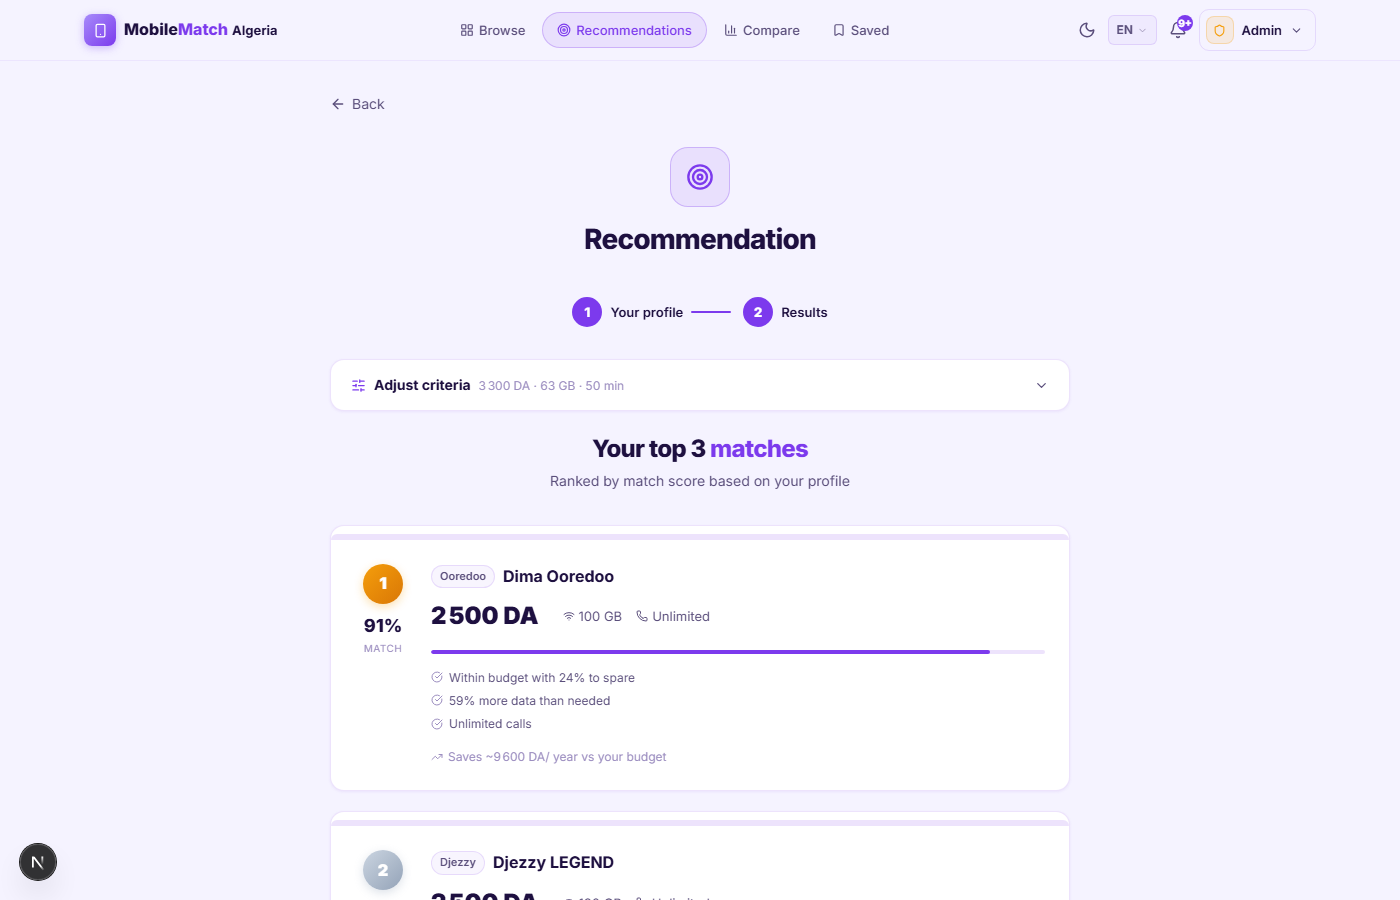
\includegraphics[width=0.95\textwidth]{images/screenshot_recommend}
  \caption{Recommendations page --- form and personalised results}
  \label{fig:ss-recommend}
\end{figure}

\subsection{Login and Registration}

Figure~\ref{fig:ss-login} shows the authentication screens. The login page accepts an email address and password; the registration page adds a name field. Both forms perform client-side validation before submitting. Incorrect credentials trigger a non-destructive inline error message without reloading the page.

\begin{figure}[H]
  \centering
  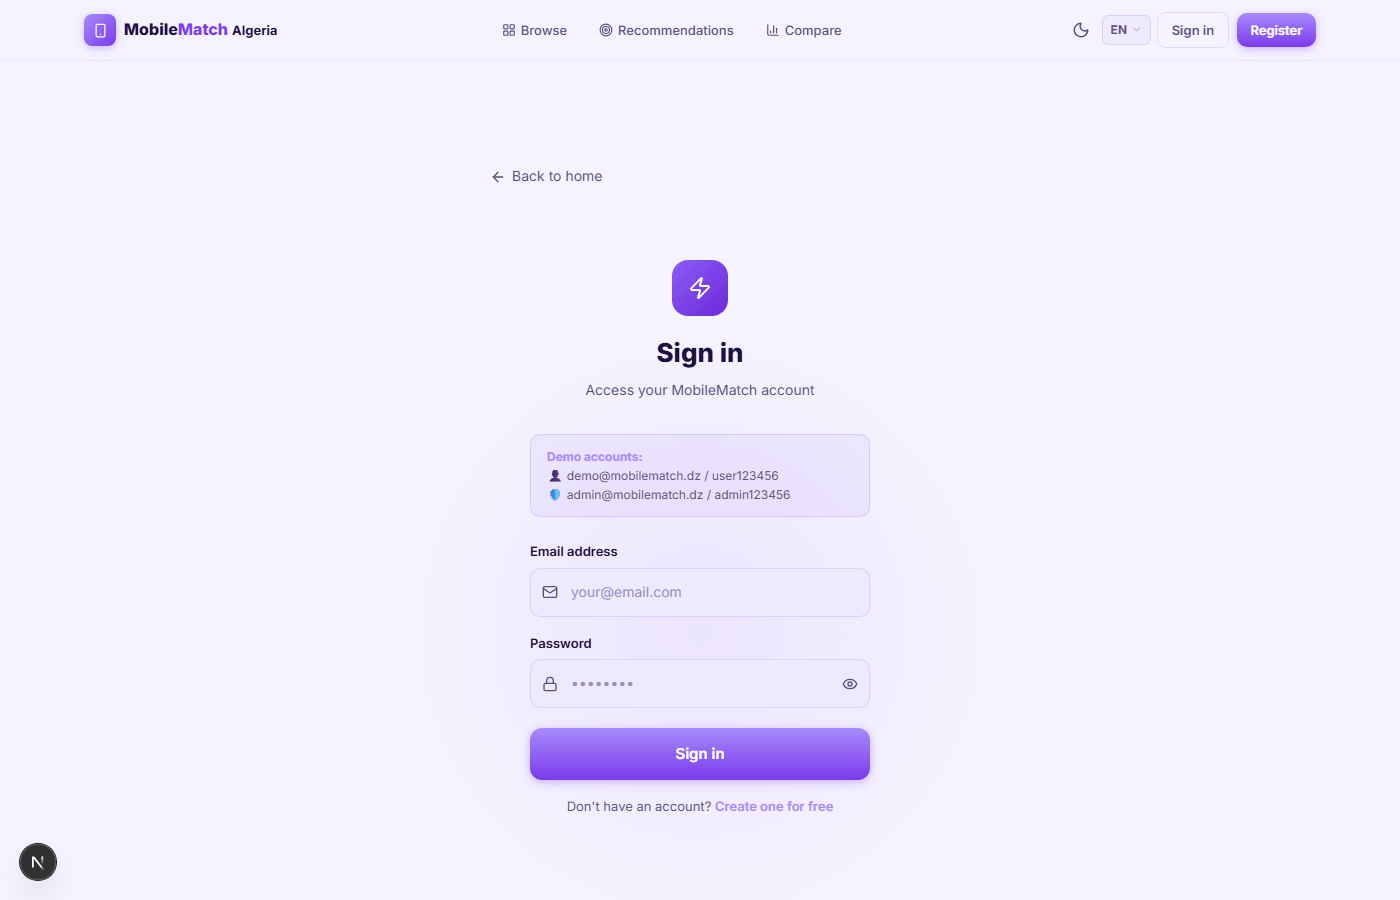
\includegraphics[width=0.95\textwidth]{images/screenshot_login}
  \caption{Login page}
  \label{fig:ss-login}
\end{figure}

\subsection{Admin Dashboard}

The admin dashboard (Figure~\ref{fig:ss-admin}) is accessible only to users with the \texttt{ADMIN} role, verified server-side on every request. It presents four statistics cards (active offers, registered users, scrape sessions, and scrape success rate), an operator health panel showing the last scrape status and offer count per operator, a per-family plan breakdown that colour-codes each scraped plan family as live, fallback, or fixed data after every run, a scrape history log with detailed per-operator event lines, and a notifications tab listing all system and recommendation alerts sent to the administrator.

\begin{figure}[H]
  \centering
  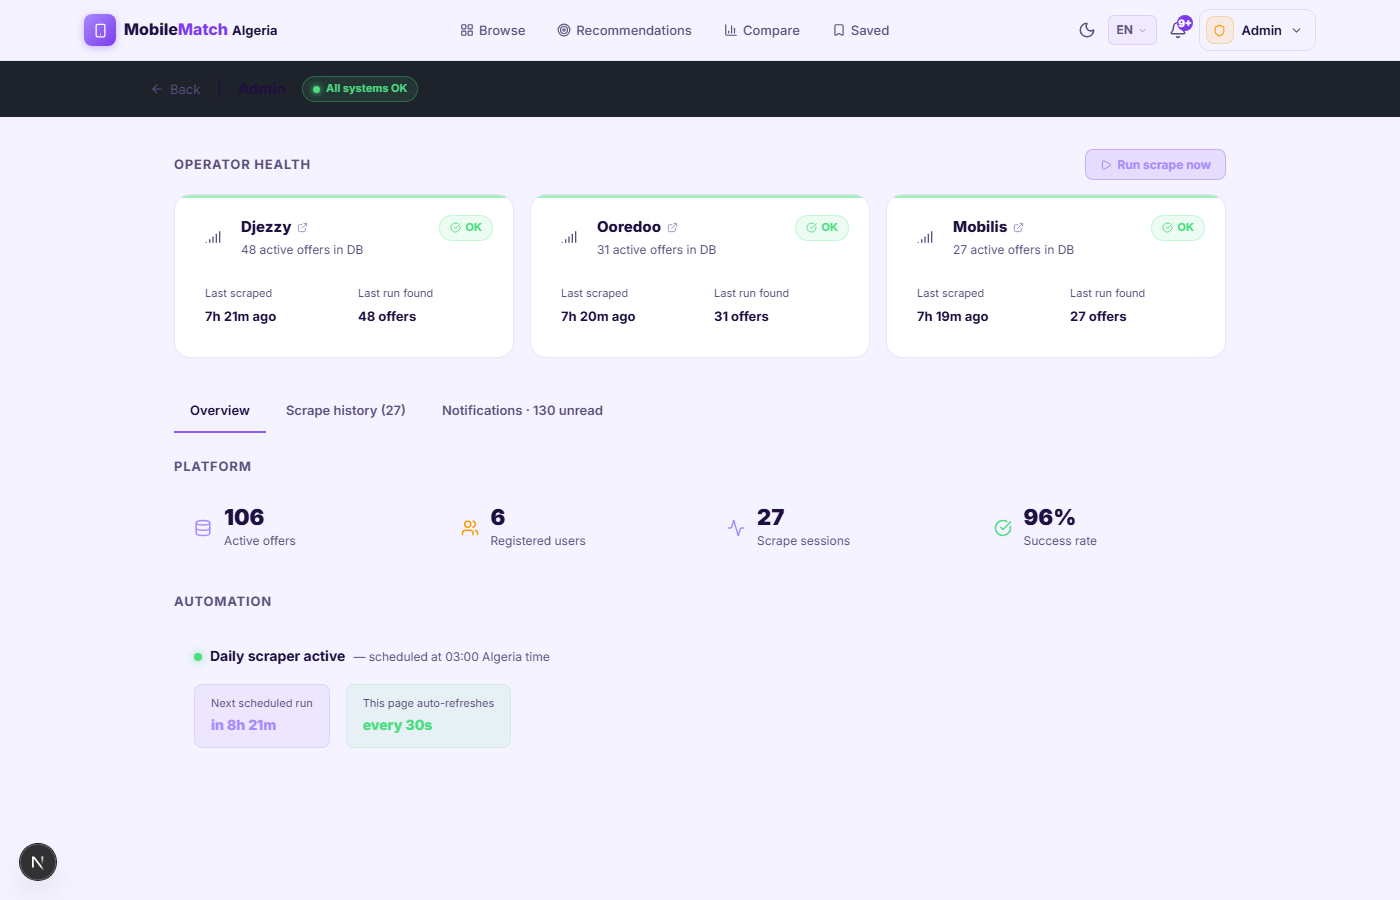
\includegraphics[width=0.95\textwidth]{images/screenshot_admin}
  \caption{Admin dashboard --- statistics, operator health panel, and scrape log}
  \label{fig:ss-admin}
\end{figure}

\section{Security}

\subsection{Authentication and Session Management}

User sessions are managed by NextAuth.js using signed JWT tokens. The secret key is stored in the \texttt{NEXTAUTH\_SECRET} environment variable. Tokens have a 30-day maximum age and are renewed on each valid request.

\subsection{Password Storage}

Passwords are hashed using bcrypt with a cost factor of 12 before being written to the database. Plain-text passwords are never logged or stored. At sign-in, \texttt{bcrypt.compare} verifies the supplied password against the stored hash without reversing the hash.

\subsection{Role-Based Access Control}

Admin-only API routes check for the \texttt{ADMIN} role in the decoded session before executing any privileged operation. A missing or non-admin session returns \texttt{401 Unauthorized} or \texttt{403 Forbidden} respectively. This check is implemented at the application layer for every relevant route handler.

\subsection{Input Validation and Injection Prevention}

All numeric query parameters are parsed and range-checked before use. All database queries are issued through Prisma's parameterised query interface, which prevents SQL injection by construction. No user-supplied string is ever interpolated directly into a query.

\section{Deployment}

{\sloppy The application is built for production with \texttt{next build}, which performs static analysis, tree-shaking, and route-level code splitting. The resulting artefact is a Node.js server launched with \texttt{next start}. Three environment variables must be set: \texttt{DATABASE\_URL} (path to the SQLite file), \texttt{NEXTAUTH\_SECRET} (JWT signing key), and \texttt{NEXTAUTH\_URL} (public base URL). The SQLite file is the only persistent artefact that must be preserved across deployments.\par}

\section*{Chapter Summary}

This chapter has described the full implementation of \textit{Mobile Match Algeria}: the development environment, the automated scraping pipeline and its per-family deactivation guard, the REST API and its cross-operator comparison routing, the multi-criteria recommendation engine with operator affinity personalisation, the eight key user interface screens, the security architecture, and the deployment configuration. Chapter~4 evaluates these implementations against the project objectives and documents the known limitations.
